\documentclass[titlepage]{jarticle}
\usepackage{h31ec-exp}
\usepackage[dvipdfmx]{graphicx}
\usepackage{here}

\title{RC直列回路と交流}
\grade{2年40番}%
\author{鷲尾 優作}
\team{}
\date{令和2年7月22日}
\expdate{令和2年7月29日}
\coauthor{%
  \\
  \\
  }

\begin{document}
\maketitle

\section{本実験の目的}
抵抗(R)とコンデンサ(C)の直列回路の電圧・電流を測定し,\\回路のインピーダンス・電流・位相について理解する.
\section{理論}
抵抗R[Ω]とコンデンサC[F]の直接接続回路は,交流に対して電流の流れを妨げる働きをする.\\
これをインピーダンスという.RC直列回路のインピーダンスZ[Ω]は,\\
Rと容量性リアクタンスXcとの代数和にならず,次式で表される.\\
\begin{eqnarray}
    Z=\sqrt{R^2+Xc^2} \nonumber \\
    =\sqrt{R^2+(\frac{1}{\omega \cdot C})} [Ω]
\end{eqnarray}

また,交流電源の電圧をv[V],RC直列回路を流れる電流をi[A]とすると,\\
\begin{eqnarray}
    i=\frac{v}{Z} [A]
\end{eqnarray}

となる.

\section{実験}
\subsection{原理}
(1)電流の大きさ\\
RC直列回路に流れる電流はRを利用して測定する.\\図2においてRC直列回路を流れる電流は,Rをも流れている.\\
したがって,Rの両端の電圧v2[V]を測定し,R[Ω]で割れば,Rを流れる電流$I_R$すなわちiがわかる.

\begin{eqnarray}
    i_R=\frac{v2}{R}\\
    i=i_R\nonumber
\end{eqnarray}

(2)電圧と電流の位相差\\
2つ以上の交流波形の時間的なずれを位相差と呼ぶ。\\位相差は交流波形の1周期を角度(360°または2π[rad])に換算し、表現する。
\begin{figure}[H]
    \begin{center}
        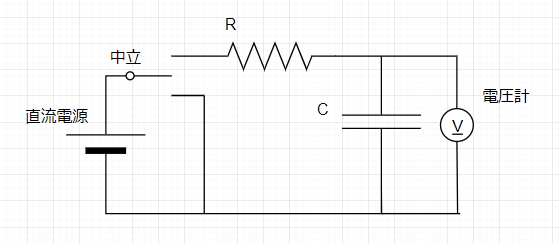
\includegraphics[width=10cm]{image/3.png}
        \caption{コンデンサの充放電特性}
    \end{center}
\end{figure}

図3を例にとると,Vに比べ,Iは右側にちょうど1目盛分ずれている.\\1周期4目盛を360°として,ずれは1周期分なのだから,
Vに対するIの位相差は次のように計算できる.

\begin{eqnarray}
    \frac{360°}{4}=90°\nonumber
\end{eqnarray}

一般に,VとIの関係のようにVに比べIが右側にある状態を,IはVに比べ,90°遅れていると表現する.

\subsection{コンデンサの電圧と電流の位相差}
コンデンサだけの回路で、コンデンサの電圧に対するコンデンサを流れる電流の位相差について測定する。\\
図2の接続図で、Rの値をXcに比べて、無視できるぐらい小さな値にすると、\\コンデンサだけの回路と考えることができる。
\subsubsection{測定}
\begin{flushleft}
    ア)図2のように接続する。\\
    イ) 抵抗 R=10[Ω] コンデンサ C=0.21[uF] 交流電圧 V=2.83[Vrms] f=1[KHz]\\
    ウ) f=1[KHz]~10[KHz]、1[KHz]間隔\\
    エ) コンデンサの電圧波形v、コンデンサの電流波形v2、として位相差を測定する\\
\end{flushleft}

\subsubsection{測定結果}
\begin{figure}[H]
    \begin{center}
        \caption{表1 コンデンサの電圧と電流の位相差}
        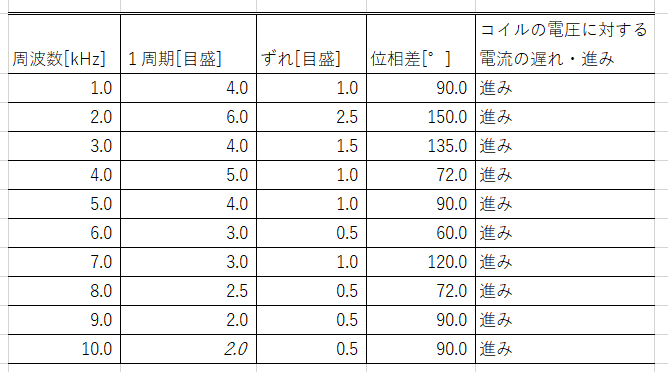
\includegraphics[width=10cm]{image/sp1.png}
    \end{center}
\end{figure}

\subsection{RC直列回路の電流・インピーダンス・位相差測定}
\subsubsection{測定}
\begin{flushleft}
    ア)図2のように接続する。\\
    イ) 抵抗 R=1000[Ω] コンデンサ C=0.05[uF] 交流電圧 V=2.83[Vrms] f=1[KHz]\\
    ウ) f=1[KHz]~10[KHz]、1[KHz]で,抵抗の電圧v2[Vrms],位相差を測定する\\
    エ) 測定結果から,電流i[Arms],インピーダンスZ[Ω]を算出する\\
\end{flushleft}

\subsubsection{測定結果}
\begin{figure}[H]
    \begin{center}
        \caption{表2 RC直列回路の電流・インピーダンス・位相差}
        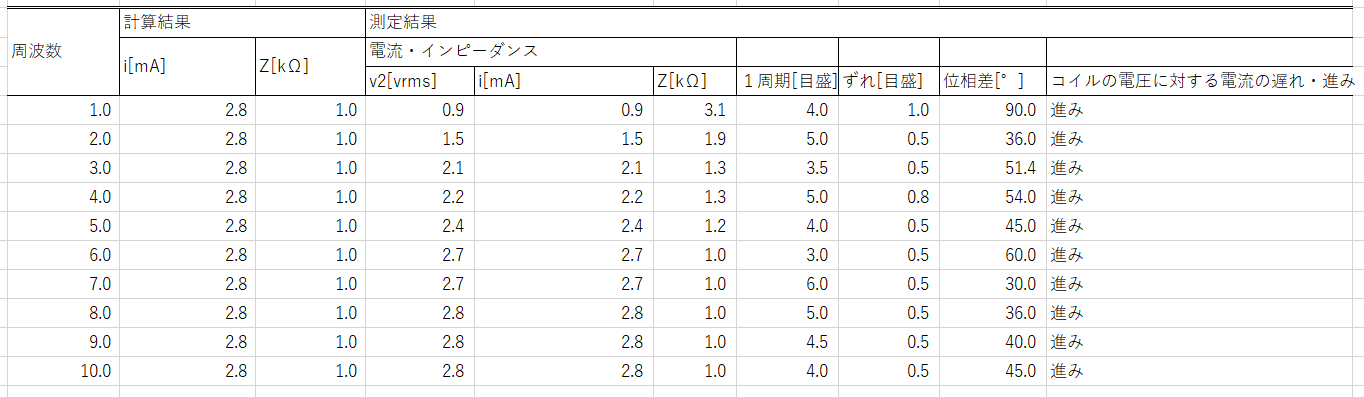
\includegraphics[width=17cm]{image/sp2.png}
    \end{center}
\end{figure}

\section{使用器具}
\begin{enumerate}
    \item 低周波発振器\\用途 交流電源確保のため\\商品名KENWOOD AG-203\\物品番号Ec-2020
    \item 抵抗器\\用途 測定対象として使用するため\\商品名DECADE RESISTOR TYPE YRH-4BA\\物品番号なし
    \item コンデンサ\\用途 測定対象として使用するため\\商品名TYPE DSC-I DECADE CAPACITOR\\物品番号帳8分類い46番号28
    \item オシロスコープ\\用途 実験データ計測のため\\商品名GW INSTEC GDS-1052-U\\物品番号DSO-20
\end{enumerate}

\section{課題考察}
\begin{enumerate}
    \item 3.2.2の測定結果から,周波数対位相差をグラフで示せ\\
          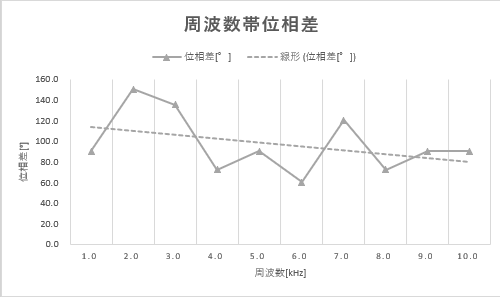
\includegraphics[width=10cm]{graph/1.png}\\
    \item 3.3.2の測定結果から,周波数対インピーダンス,周波数対位相差をグラフで示せ\\
          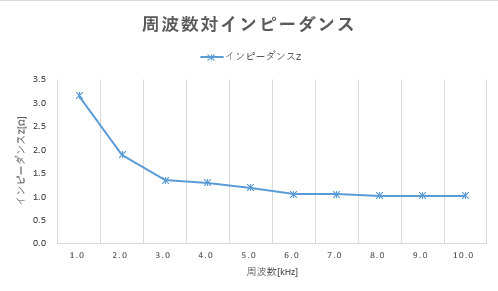
\includegraphics[width=10cm]{graph/2.png}\\
          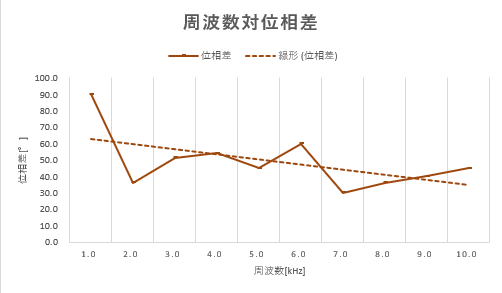
\includegraphics[width=10cm]{graph/3.png}\\
    \item 3.3.2の測定結果から,コンデンサの電圧とコンデンサを流れる電流について言えることは何か.教科書等を参考に述べよ\\
          コンデンサにおいて,電圧と電流の関係は以下のようになる
          \begin{eqnarray}
              i=\frac{v}{Z} [A]
          \end{eqnarray}
          3.3.2の表,グラフからも読み取れるよう,実験結果は周波数が増加すると\\
          インピーダンスが減少しており,式は成立している.
    \item 3.3.2の測定結果の測定結果において,電流の大きさ,インピーダンスについて,計算値と測定結果を比較せよ\\
          3.3.2において,電流の大きさ,インピーダンスは計算と同一になったものが多かった\\
          しかし,低周波数域において誤差が増加しており,実験ミスによるものなのか\\
          その他原因があるのかは判断できなかった.
\end{enumerate}


\section{感想}
実験当日欠席し,別日に再実験となり,一人での作業となった.\\
操作が非常に多く記録と同時並行で行うことに大変苦労したがなんとか完了できた.\\
分担の大切さを感じた.
\end{document}